\documentclass[a4paper,12pt, oneside]{book}

%\usepackage{fullpage}
\usepackage[T1]{fontenc}
\usepackage[italian]{babel}
\usepackage[utf8]{inputenc}
\usepackage{amssymb}
\usepackage{amsthm}
\usepackage{graphics}
\usepackage{amsfonts}
\usepackage{listings}
\usepackage{amsmath}
\usepackage{amstext}
\usepackage{engrec}
\usepackage{rotating}
\usepackage[safe,extra]{tipa}
\usepackage{showkeys}
\usepackage{multirow}
\usepackage{hyperref}
\usepackage{microtype}
\usepackage{enumerate}
\usepackage{braket}
\usepackage{marginnote}
\usepackage{pgfplots}
\usepackage{cancel}
\usepackage{polynom}
\usepackage{booktabs}
\usepackage{enumitem}
\usepackage{framed}
\usepackage{pdfpages}
\usepackage{pgfplots}
\usepackage[cache=false]{minted}
 \usepackage[usenames,dvipsnames, pdf]{pstricks}
 \usepackage{epsfig}
 \usepackage{pst-grad} % For gradients
 \usepackage{pst-plot} % For axes
 \usepackage[space]{grffile} % For spaces in paths
 \usepackage{etoolbox} % For spaces in paths
 \makeatletter % For spaces in paths
 \patchcmd\Gread@eps{\@inputcheck#1 }{\@inputcheck"#1"\relax}{}{}
 \makeatother
\usepackage{fancyhdr}
\pagestyle{fancy}
\fancyhead[LE,RO]{\slshape \rightmark}
\fancyhead[LO,RE]{\slshape \leftmark}
\fancyfoot[C]{\thepage}



\title{Analisi e Progettazione del Software}
\author{UniShare\\\\Davide Cozzi\\\href{https://t.me/dlcgold}{@dlcgold}\\\\Gabriele De Rosa\\\href{https://t.me/derogab}{@derogab} \\\\Federica Di Lauro\\\href{https://t.me/f_dila}{@f\textunderscore dila}}
\date{}

\pgfplotsset{compat=1.13}
\begin{document}
\maketitle

\definecolor{shadecolor}{gray}{0.80}

\newtheorem{teorema}{Teorema}
\newtheorem{definizione}{Definizione}
\newtheorem{esempio}{Esempio}
\newtheorem{corollario}{Corollario}
\newtheorem{lemma}{Lemma}
\newtheorem{osservazione}{Osservazione}
\newtheorem{nota}{Nota}
\newtheorem{esercizio}{Esercizio}
\tableofcontents
\renewcommand{\chaptermark}[1]{%
\markboth{\chaptername
\ \thechapter.\ #1}{}}
\renewcommand{\sectionmark}[1]{\markright{\thesection.\ #1}}
\chapter{Introduzione}
\textbf{Questi appunti sono presi durante le lezioni in aula. Per quanto sia stata fatta una revisione è altamente probabile (praticamente certo) che possano contenere errori, sia di stampa che di vero e proprio contenuto. Per eventuali proposte di correzione effettuare una pull request. Link: } \url{https://github.com/dlcgold/Appunti}.\\
\textbf{Grazie mille e buono studio!}
\chapter{Introduzione all'Ingegneria del software}
Durante il corso di Analisi e Progettazione del software si analizzano i modelli e i principi per lo sviluppo di un 
ottimo e ben mantenibile software, andando anche ad analizzare, in maniera sommaria, anche tutti gli strumenti di 
ingegneria del software, necessari per lo sviluppo ottimale di un software.

In questo corso studieremo in dettaglio i seguenti argomenti:
\begin{itemize}
\item introduzione all'ingegneria del software
\item progettazione sistemi orientati ad oggetti
\item modellazione a dominio
\item UML e analisi dei casi d'uso
\item design pattern
\item sviluppo test-driven(cenni)
\item code smell e refactoring(cenni)
\end{itemize}
Il software, è l'insieme delle componenti modificabili e non fisiche di un calcolatore elettronico
e si può intendere anche come un programma eseguibile, viene diviso in due categorie:
\begin{itemize}
\item generici, per un ampio range di clienti, come ad esempio gli elaboratori di testi
\item custom, per un singolo cliente, come ad esempio i gestionali specifici di un impresa
\end{itemize}
Nello sviluppo di software si utlizza spesso una base pre-esistente, infatti l'ingegneria del software si occupa
di tutti gli aspetti per lo sviluppo del software, sfruttando di solito una base preesistente. \newline
Di solito quando si sviluppa un software si presuppone che abbia una durata di alcuni anni, con la predispozione
al cambiamento e all'introduzione di nuove features infatti un software per essere utile deve essere continuamente cambiato.

Si hanno due tipologie di progetti:
\begin{enumerate}
\item progetti di routine, soluzione di problemi e riuso di vecchio codice
\item progetti innovativi, soluzioni nuovi
\end{enumerate}
e solitamente l'ingegneria del software si occupa principalmente di progetti innovativi 
con specifiche del progetto variabili, con la presenza di cambiamenti continui e ovviamente 
non è uguale nè similare con l'ingegneria tradizionale.

Un programmatore normalmente lavora da solo, su un programma completo con specifiche note mentre un ingegnere del software
lavora in gruppo, progetta componenti e l'architettura e identifica requisiti e specifiche.
Il costo del software spesso supera quello hardware %aggiungere grafico

Nello sviluppo di un software si hanno le seguenti fasi di sviluppo:
\begin{itemize}
\item \textbf{analisi dei requisiti}, che indica cosa deve fare il sistema
\item \textbf{progettazione}, progetto del sistema d implementare 
\item \textbf{sviluppo}, produzione del sistema software
\item \textbf{convalida}, verifica dei requisiti del cliente
\item \textbf{evoluzione}, evoluzione al cambiare di requisiti del cliente
\end{itemize} 
Si hanno dei sistemi software per l'automazione delle attività svolte nel progetto software, 
questi sono i cosiddetti \textbf{CASE (\textit{Computer-Aided Software Engineering})} che si dividono in:
\begin{description}
    \item [CASE di alto livello] per il supporto alle prime attività di processo come la raccolta requisiti e la progettazione
    \item [CASE di basso livello] per il supporto alle ultime attività di processo come la programmazione,
                                  il debugging, testing e reverse engineering
\end{description}
Il software, oltre a fornire quanto richiesto dal cliente, deve essere:
\begin{itemize}
\item \textbf{mantenibile}, quindi semplice da mantenere ed aggiornare
\item \textbf{affidabile}, quindi con bassa possibilità di malfunzionamenti
\item \textbf{efficiente}, quindi deve fare buon uso delle risorse
\item \textbf{facilmente usabile}
\end{itemize}
Il software deve essere accettato dagli utenti per i quali è stato sviluppato per cui deve essere comprensibile, 
usabile e compatibile con altri sistemi.
Esiste un codice etico, \textbf{ACM/IEEE}, con otto principi legati al comportamento degli ingegneri del software.\\
Un \textbf{sistema} è una collezione significativa di componenti interrelati che lavorano assieme per realizzare
un obiettivo comune quindi include software e parti meccaniche o elettriche.
Si ha inoltre che i vari componenti possono dipendere da altri componenti e che le proprietà
e il comportamento dei vari componenti sono intrinsecamente correlati, quindi si hanno due macro categorie:
\begin{enumerate}
    \item \textbf{sistemi tecnico-informatici} con le seguenti caratteristiche:
    \begin{itemize}
        \item includono hardware e software
        \item non includono gli operatori e i processi operazionali
        \item il sistema non conosce lo scopo del suo utilizzo
        \item si hanno \textbf{proprietà emergenti:}
        \begin{itemize}
            \item le proprietà del sistema finale dipendono dalle sue componenti e dalle relazioni tra le componenti
            \item queste proprietà possono essere misurate solamente sul sistema finale
        \end{itemize}
        \item si ha il \textbf{non-determinismo}, ovvero il sistema non risponde sempre con lo stesso output dato lo
              stesso input perché il risultato è spesso dipendente dal comportamento degli operatori umani
        \item si ha un complesso legame tra i sistemi e gli obbiettivi aziendali, ovvero l'efficacia nel supportare
                gli obiettivi aziendali non dipende solo dal sistema stesso
    \end{itemize}
    \item \textbf{sistemi socio-tecnici} con le seguenti caratteristiche:
    \begin{itemize}
        \item includono uno o più sistemi tecnici, ma anche i processi operazionali e gli operatori
        \item sono fortemente condizionati da politiche aziendali e regole
\end{itemize}
\end{enumerate}
\newpage
Vediamo qualche proprietà emergente:
\begin{itemize}
\item \textbf{volume:} il volume di un sistema (lo spazio totale occupato) varia a seconda di come sono
disposti e collegati i componenti che lo formano
\item \textbf{affidabilità:} l'affidabilità del sistema dipende dall'affidabilità dei componenti, ma interazioni
impreviste possono produrre nuovi fallimenti e quindi influenzare l'affidabilità dell'intero sistema
\item \textbf{protezione:} la protezione del sistema (la sua abilità di resistere agli attacchi) è una proprietà
complessa che non può essere facilmente misurata. Possono essere inventati nuovi attacchi che non erano stati previsti dai progettisti del sistema, in modo da abbattere le difese integrate
\item \textbf{riparabilità:} questa proprietà riflette la facilità con cui è possibile correggere un problema del
sistema quando questo viene scoperto; dipende dalla possibilità di diagnosticare il problema, di accedere ai componenti difettosi e di modificarli o sostituirli
\item \textbf{usabilità:} questa proprietà mostra la facilità d‘uso del sistema e dipende dai componenti del
sistema tecnico, dai suoi operatori e dal suo ambiente operativo
\end{itemize}
Si hanno poi le proprietà del tipo \textit{"non deve accadere"}:
\begin{itemize}
\item prestazioni o affidabilità possono essere misurate
\item altre proprietà sono solo comportamenti che \underline{\textbf{non devono accadere}}; si hanno due tematiche:
\begin{enumerate}
\item \textbf{sicurezza:} il sistema non deve causare danni a
persone o all'ambiente
\item \textbf{protezione: }il sistema non deve permettere utilizzi non autorizzati
\end{enumerate}
\end{itemize}
I sistemi Socio-tecnici sono sistemi pensati per
raggiungere obiettivi aziendali o organizzativi e bisogna comprendere a fondo l'ambiente organizzatico nel quale un certo sistema è usato
\subsection{Sistemi Critici}
Abbiamo tre esempi di sistemi critici:
\begin{enumerate}
\item \textbf{sistemi safety-critical} dove i fallimenti comportano rischi ambientali o perdite di vite umane (per esempio un sistema di controllo per un impianto chimico)
\item \textbf{sistemi mission-critical} dove i fallimenti possono causare il fallimento di attività a obiettivi
diretti (per esempio un sistema di navigazione di un veicolo spaziale)
\item \textbf{sistemi business-critical} dove i fallimenti possono risultare in perdite di denaro sostenute (per esempio un sistema bancario)
\end{enumerate}
Ci possono essere vari fallimenti:
\begin{itemize}
\item \textbf{fallimenti hardware}, errori di progetto, produzione o "consumo"
\item \textbf{fallimenti software}, errori di specifica, progetto, implementazione
\item \textbf{errori operativi}, errori commessi da operatori umani (forse una delle maggiori cause di fallimenti)
\end{itemize}
Nei sistemi critici, generalmente la fidatezza è la più importante proprietà del sistema in quanto si ha un alto costo dei fallimenti. La fidatezza riflette il livello di confidenza che l'utente ha verso il sistema. \textbf{Utilità e fidatezza non sono la stessa cosa}. Possiamo elencare delle proprietà della fidatezza.
\begin{itemize}
\item \textbf{disponibilità}, ovvero la capacità del sistema di fornire servizi quando richiesto
\item \textbf{affidabilità}, ovvero la capacità del sistema
di fornire servizi come specificato
\item \textbf{sicurezza}, ovvero la capacità del sistema di
lavorare senza rischiare fallimenti catastrofici
\item \textbf{protezione}, ovvero la capacità del sistema
di proteggersi contro intrusioni accidentali o volontarie
\item \textbf{riparabilità}, ovvero la facilità con cui un sistema può essere riparato in caso di fallimenti
\item \textbf{mantenibilità}, ovvero la facilità con cui un sistema può essere adattato a nuovi requisiti
\item \textbf{sopravvivenza}, ovvero la capacità del sistema di fornire servizi anche se sotto attacco
\item \textbf{tolleranza dell'errore}, ovvero fino a che punto il sistema riesce a tollerare o evitare errori di immissione 
\end{itemize}
Il costo dei fallimenti nei sistemi critici è così alto che i metodi di ingegneria del software non sono cost-effective per i sistemi non critici. D'altro canto i costi della fidatezza incrementano esponenzialmente all'aumentare del livello di fidatezza richiesto, per due ragioni principali:
\begin{enumerate}
\item l'uso di tecniche di sviluppo più costose ed hardware di alta affidabilità
\item l'aumentare del tempo dedicato al testing ed analisi per convalidare la raggiunta fidatezza.
\end{enumerate}
A causa del costo di un sistema dotato di elevata fidatezza, potrebbe essere conveniente sviluppare un sistema non fidato e pagare per i costi dei fallimenti; questa scelta dipende da fattori sociali e politici. La scelta finale dipende sempre dal sistema, per un normale sistema di business una fidatezza
moderata può essere sufficiente
\subsection{Modelli di Processo}
Il modello di un processo software è una rappresentazione
semplificata del processo. Questa rappresentazione è basata su un aspetto specifico:
\begin{itemize}
\item \textbf{modello a flusso di lavoro (Workflow)} per una sequenza di attività
\item \textbf{modello a flusso di dati (Data-flow)} per il flusso delle informazioni
\item \textbf{modello ruolo/azione (role/action)} per decidere i vari ruoli
\end{itemize}
si hanno poi tre modelli generici:
\begin{enumerate}
\item \textbf{modello a cascata (waterfall)}
\item \textbf{modello ciclico (Iterative development)}
\item \textbf{ingegneria del Software basata sui componenti (CBSE)}
\end{enumerate}
Con i metodi di ingegneria del software su ha un approccio strutturato allo sviluppo software (quali modelli utilizzare e quando, convenzioni sulla notazione, vincoli sui
modelli. per esempio  id univoco alle entità raccomandazioni, o conformità ad un certo stile progettuale guida al processo). Si passa quindi da un modello di processo ad un metodo:
\begin{center}
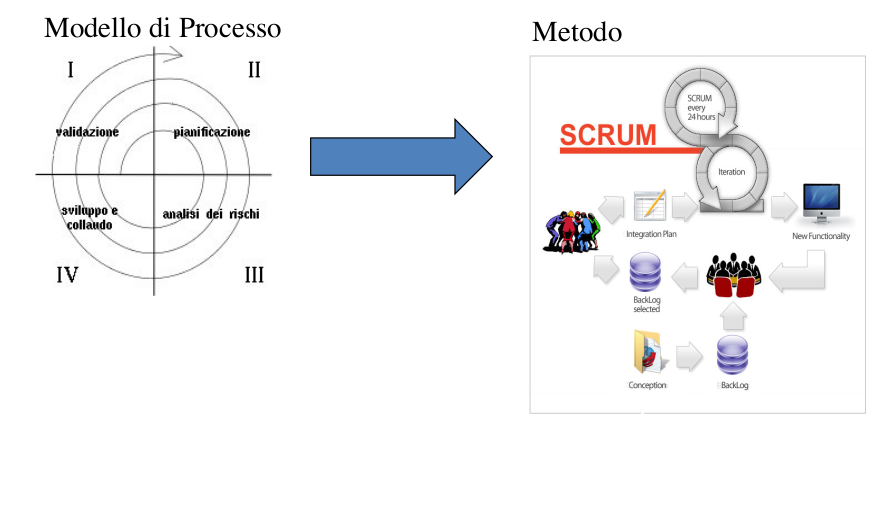
\includegraphics[scale=2.0]{img/ing.png}
\end{center}
Si ha il modello a cascata, inventato da Royce:
\begin{center}
\psscalebox{1.0 1.0} % Change this value to rescale the drawing.
{
\begin{pspicture}(0,-3.755)(9.11,3.755)
\rput[bl](0.0,3.445){feasibilty study}
\rput[bl](1.2,2.245){requirements analysis \& specification}
\rput[bl](2.8,1.045){design}
\rput[bl](3.6,-0.155){coding \& unit test}
\rput[bl](4.4,-1.355){integration \& system test}
\rput[bl](6.0,-2.555){deployment}
\rput[bl](7.2,-3.755){maintenance}
\psline[linecolor=black, linewidth=0.04, arrowsize=0.05291667cm 2.0,arrowlength=1.4,arrowinset=0.0]{->}(1.2,3.445)(2.0,2.645)
\psline[linecolor=black, linewidth=0.04, arrowsize=0.05291667cm 2.0,arrowlength=1.4,arrowinset=0.0]{->}(2.4,2.245)(3.2,1.445)
\psline[linecolor=black, linewidth=0.04, arrowsize=0.05291667cm 2.0,arrowlength=1.4,arrowinset=0.0]{->}(3.6,1.045)(4.4,0.245)
\psline[linecolor=black, linewidth=0.04, arrowsize=0.05291667cm 2.0,arrowlength=1.4,arrowinset=0.0]{->}(4.8,-0.155)(5.6,-0.955)
\psline[linecolor=black, linewidth=0.04, arrowsize=0.05291667cm 2.0,arrowlength=1.4,arrowinset=0.0]{->}(6.0,-1.355)(6.8,-2.155)
\psline[linecolor=black, linewidth=0.04, arrowsize=0.05291667cm 2.0,arrowlength=1.4,arrowinset=0.0]{->}(7.2,-2.555)(8.0,-3.355)
\end{pspicture}
}
\end{center}
\newpage
si ha il seguente feedback del modello a cascata:
\begin{center}
\psscalebox{1.0 1.0} % Change this value to rescale the drawing.
{
\begin{pspicture}(0,-3.8)(15.6,3.8)
\psframe[linecolor=black, linewidth=0.04, dimen=outer](2.8,3.8)(0.0,2.6)
\psframe[linecolor=black, linewidth=0.04, dimen=outer](6.0,2.2)(2.8,1.0)
\psframe[linecolor=black, linewidth=0.04, dimen=outer](9.2,0.6)(6.0,-0.6)
\psframe[linecolor=black, linewidth=0.04, dimen=outer](12.4,-1.0)(9.2,-2.2)
\psframe[linecolor=black, linewidth=0.04, dimen=outer](15.6,-2.6)(12.4,-3.8)
\rput[bl](0.53333336,3.3){definizione}
\rput[bl](0.43333334,2.82){dei requisiti}
\rput[bl](2.8990476,1.76){progettazione}
\rput[bl](3.1866667,1.46){del sistema e}
\rput[bl](6.087619,0.0){implementazione}
\rput[bl](6.0804764,-0.44){e test delle unità}
\rput[bl](9.546667,-1.52){integrazione e }
\rput[bl](9.486667,-2.0){test del sistema}
\rput[bl](13.066667,-3.22){operatività}
\rput[bl](12.646667,-3.5){e manutenzione}
\rput[bl](3.58,1.14){del software}
\psline[linecolor=black, linewidth=0.04, arrowsize=0.05291667cm 2.0,arrowlength=1.4,arrowinset=0.0]{->}(12.4,-3.4)(1.2,-3.4)(1.2,2.6)
\psline[linecolor=black, linewidth=0.04, arrowsize=0.05291667cm 2.0,arrowlength=1.4,arrowinset=0.0]{->}(10.8,-3.4)(10.8,-2.2)
\psline[linecolor=black, linewidth=0.04, arrowsize=0.05291667cm 2.0,arrowlength=1.4,arrowinset=0.0]{->}(7.6,-3.4)(7.6,-0.6)
\psline[linecolor=black, linewidth=0.04, arrowsize=0.05291667cm 2.0,arrowlength=1.4,arrowinset=0.0]{->}(4.4,-3.4)(4.4,1.0)
\psline[linecolor=black, linewidth=0.04, arrowsize=0.05291667cm 2.0,arrowlength=1.4,arrowinset=0.0]{->}(2.8,3.4)(4.4,3.4)(4.4,2.2)
\psline[linecolor=black, linewidth=0.04, arrowsize=0.05291667cm 2.0,arrowlength=1.4,arrowinset=0.0]{->}(6.0,1.8)(7.6,1.8)(7.6,0.6)
\psline[linecolor=black, linewidth=0.04, arrowsize=0.05291667cm 2.0,arrowlength=1.4,arrowinset=0.0]{->}(9.2,0.2)(10.8,0.2)(10.8,-1.0)
\psline[linecolor=black, linewidth=0.04, arrowsize=0.05291667cm 2.0,arrowlength=1.4,arrowinset=0.0]{->}(12.4,-1.4)(14.0,-1.4)(14.0,-2.6)
\end{pspicture}
}
\end{center}
I requisiti di sistema evolvono \textbf{sempre} durante il corso del progetto.\\
Quindi il modello a cascata è così ben rappresentabile:
\begin{center}

\psscalebox{1.0 1.0} % Change this value to rescale the drawing.
{
\begin{pspicture}(0,-2.55)(6.71,2.55)
\rput[bl](0.0,2.25){requirements}
\rput[bl](1.6,1.05){design}
\rput[bl](2.4,-0.15){implementation}
\rput[bl](4.0,-1.35){verification}
\rput[bl](4.8,-2.55){maintenance}
\psline[linecolor=black, linewidth=0.04, arrowsize=0.05291667cm 2.0,arrowlength=1.4,arrowinset=0.0]{->}(1.2,2.25)(2.0,1.45)
\psline[linecolor=black, linewidth=0.04, arrowsize=0.05291667cm 2.0,arrowlength=1.4,arrowinset=0.0]{->}(2.4,1.05)(3.2,0.25)
\psline[linecolor=black, linewidth=0.04, arrowsize=0.05291667cm 2.0,arrowlength=1.4,arrowinset=0.0]{->}(3.6,-0.15)(4.4,-0.95)
\psline[linecolor=black, linewidth=0.04, arrowsize=0.05291667cm 2.0,arrowlength=1.4,arrowinset=0.0]{->}(4.8,-1.35)(5.6,-2.15)
\end{pspicture}
}

\end{center}
Invece di rilasciare il sistema in una singola consegna,
sviluppo e consegna sono strutturati in una sequenza di
incrementi, ognuno dei quali corrispondenti a parte
delle funzionalità richieste. Questa è la \textbf{consegna incrementale}. requisiti utente sono ordinati per priorità, i requisiti ad alta priorità sono inclusi nei primi incrementi.  \newpage
Una volta che lo sviluppo di un incremento inizia, i
requisiti sono congelati; invece possono evolvere i
requisiti per gli incrementi successivi:
\begin{center}
\psscalebox{1.0 1.0} % Change this value to rescale the drawing.
{
\begin{pspicture}(0,-2.8)(16.05,2.8)
\rput[bl](0.4,2.4){definizione}
\rput[bl](0.4,2.0){sommaria}
\rput[bl](0.4,1.6){dei requisiti}
\rput[bl](4.4,2.4){assegnazione}
\rput[bl](4.4,2.0){dei requisiti}
\rput[bl](4.4,1.6){agli incrementi}
\rput[bl](8.8,2.4){progettazione}
\rput[bl](8.8,2.0){architettura}
\rput[bl](8.8,1.6){di sistema}
\rput[bl](0.4,-0.4){sviluppo}
\rput[bl](0.4,-0.8){degli incrementi}
\rput[bl](0.4,-1.2){di sistema}
\rput[bl](4.8,-0.4){convalida}
\rput[bl](4.8,-0.8){dell'incremento}
\rput[bl](9.2,-0.4){integrazione}
\rput[bl](9.2,-0.8){dell'incremento}
\rput[bl](13.6,-0.4){validazione}
\rput[bl](13.6,-0.8){del sistema}
\rput[bl](14.0,1.6){sistema finale}
\rput[bl](6.8,-2.8){sistema incompleto}
\psframe[linecolor=black, linewidth=0.04, dimen=outer](2.8,2.8)(0.0,1.2)
\psframe[linecolor=black, linewidth=0.04, dimen=outer](7.2,2.8)(4.0,1.2)
\psframe[linecolor=black, linewidth=0.04, dimen=outer](11.2,2.8)(8.4,1.2)
\psframe[linecolor=black, linewidth=0.04, dimen=outer](3.2,0.0)(0.0,-1.6)
\psframe[linecolor=black, linewidth=0.04, dimen=outer](7.6,0.0)(4.4,-1.6)
\psframe[linecolor=black, linewidth=0.04, dimen=outer](12.0,0.0)(8.8,-1.6)
\psframe[linecolor=black, linewidth=0.04, dimen=outer](16.0,0.0)(13.2,-1.6)
\psline[linecolor=black, linewidth=0.04, arrowsize=0.05291667cm 2.0,arrowlength=1.4,arrowinset=0.0]{->}(2.8,2.0)(4.0,2.0)
\psline[linecolor=black, linewidth=0.04, arrowsize=0.05291667cm 2.0,arrowlength=1.4,arrowinset=0.0]{->}(7.2,2.0)(8.4,2.0)
\psline[linecolor=black, linewidth=0.04, arrowsize=0.05291667cm 2.0,arrowlength=1.4,arrowinset=0.0]{->}(10.0,1.2)(10.0,0.8)(1.2,0.8)(1.2,0.0)
\psline[linecolor=black, linewidth=0.04, arrowsize=0.05291667cm 2.0,arrowlength=1.4,arrowinset=0.0]{->}(3.2,-0.8)(4.4,-0.8)
\psline[linecolor=black, linewidth=0.04, arrowsize=0.05291667cm 2.0,arrowlength=1.4,arrowinset=0.0]{->}(7.6,-0.8)(8.8,-0.8)
\psline[linecolor=black, linewidth=0.04, arrowsize=0.05291667cm 2.0,arrowlength=1.4,arrowinset=0.0]{->}(12.0,-0.8)(13.2,-0.8)
\psline[linecolor=black, linewidth=0.04, arrowsize=0.05291667cm 2.0,arrowlength=1.4,arrowinset=0.0]{->}(14.8,-1.6)(14.8,-2.4)(2.0,-2.4)(2.0,-1.6)
\psline[linecolor=black, linewidth=0.04, arrowsize=0.05291667cm 2.0,arrowlength=1.4,arrowinset=0.0]{->}(14.8,0.0)(14.8,1.6)
\end{pspicture}
}

\end{center}
Con la consegna incrementale si hanno i seguenti vantaggi:
\begin{itemize}
\item funzioni utili per il cliente possono essere rilasciate ad ogni incremento, quindi alcune funzionalità di sistema sono disponibili sin dai primi incrementi
\item i primi incrementi rappresentano dei prototipi che supportano la scoperta dei requisiti per i successivi incrementi
\item i rischi di fallimento si abbassano
\item i servizi a priorità più alta tendono ad essere collaudati più a fondo
\end{itemize}
Se si ha che i requisiti vengono scoperti attraverso lo sviluppo si ha lo \textbf{sviluppo evoluzionistico}. Si usano prototipi che poi non verranno utilizzati nel corso del progetto vero e proprio\\
\begin{center}
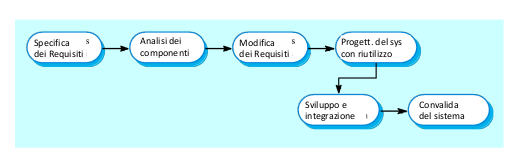
\includegraphics[scale=0.7]{img/ms.png}
\end{center}
Si ha ingegneria del software basata su componenti se si hanno già librerie su cui lavorare.\\
Passiamo al primo modello iterativo, quello di B. Boehm.
\begin{center}
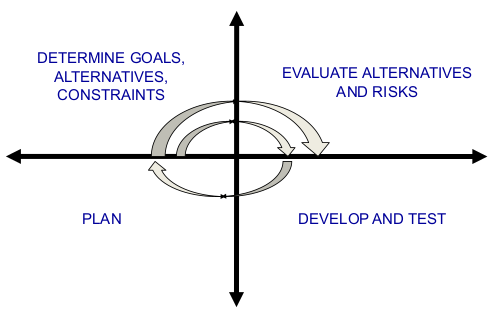
\includegraphics[scale=0.7]{img/ms2.png}
\end{center}
si parte dal quadrante in alto a sinistra e si arriva al prodotto finale mediante una serie di iterazioni. Si sceglie ovviamente la soluzione più sicura. I vari passaggi sono qui rappresentati:
\begin{center}
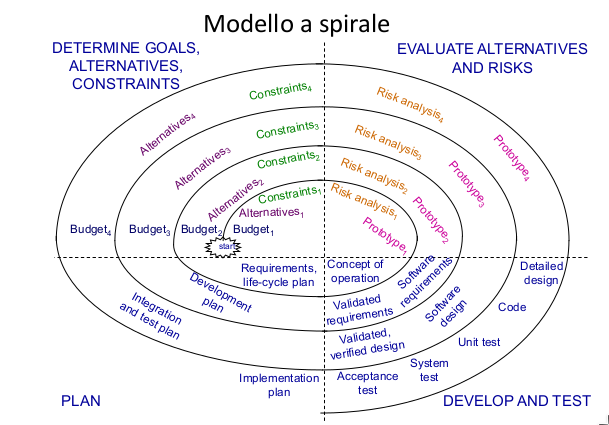
\includegraphics[scale=0.7]{img/ms3.png}
\end{center}
\section{Modelli agili}
Si hanno i modelli agili, che si basano sulla \textbf{consegna incrementale}. Si hanno iterazioni brevi e timeboxed, con un raffinamento evolutivo di piani, dei requisiti e del progetto. Questi metodi favoriscono la collaborazione nei gruppi e la riduzione dei costi.
\subsection{Modello UP o RUP}
Il metodo UP, \textit{inified process}, conosciuto anche come RUP, \textit{Rational Unified Process}, usa la notazione UML, \textit{unified modeling language} ed è uno dei più importanti modelli agili. È è un processo iterativo e incrementale. Si basa sulla suddivisone di un grande processo in iterazioni controllate. Si hanno passi piccoli, timeboxed da 2 a 6 settimane, feedback rapito e adattamento, di requisiti, modelli, stime di sviluppo e costi e priorità.
\begin{center}
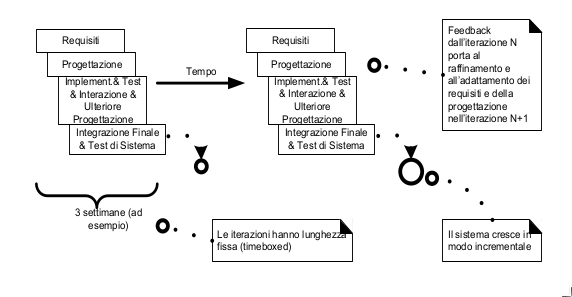
\includegraphics[scale=0.7]{img/ms4.png}
\end{center}
Si hanno 4 fasi nel modello RUP:
\begin{enumerate}
\item \textbf{avviamento:} dove viene stabilita la “bussines rationale” del progetto e stabiliti gli obiettivi, stime dei costi e dei tempi. Si ha uno studio di fattibilità, \textit{Life-Cycle Objective Milestone}
\item \textbf{elaborazione}: dove si raccolgono i requisiti in modo più dettagliato, si procede con l'analisi ad alto livello per stabilire l'architettura di base e vengono analizzati i rischi principali. Si hanno stime più affidabili: \textit{Life-Cycle Architecture Milestone}
\item \textbf{costruzione} che consiste di molte iterazioni, e ad ogni iterazione viene costruita una parte del sistema che soddisfa un sottoinsieme di requisiti. Viene effettuato il testing e l'integrazione. Si ha la preparazione al rilascio: \textit{Initial Operational Capability Milestone}
\item \textbf{transizione:} dove vengono affrontati tutti gli aspetti legati al fine-tuning delle funzionalità,
prestazioni, qualità, beta-testing, ottimizzazione, formazione degli
utenti,... È la \textit{Product Release Milestone}
\end{enumerate}
\begin{center}
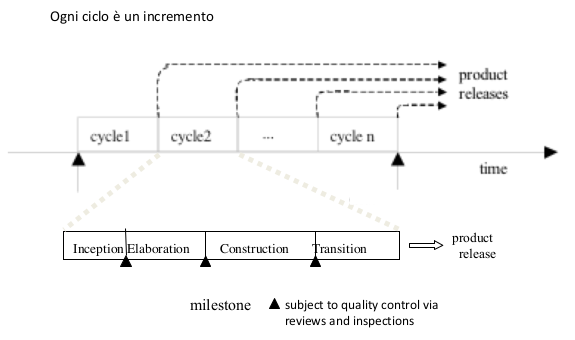
\includegraphics[scale=0.7]{img/ms5.png}
\end{center}
Si hanno i seguenti vantaggi dello sviluppo iterativo:
\begin{itemize}
\item minore chance di fallimento del progetto
\item riduzione precoce dei rischi
\item progresso visibile
\item feedback precoce e coinvolgimento dell'utente
\item "abbracciare il cambiamento"
\end{itemize}
\begin{center}
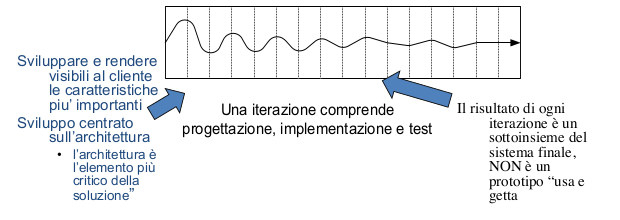
\includegraphics[scale=0.7]{img/ms6.png}
\end{center}
Vediamo un esempio con 5 iterazioni:
\begin{center}
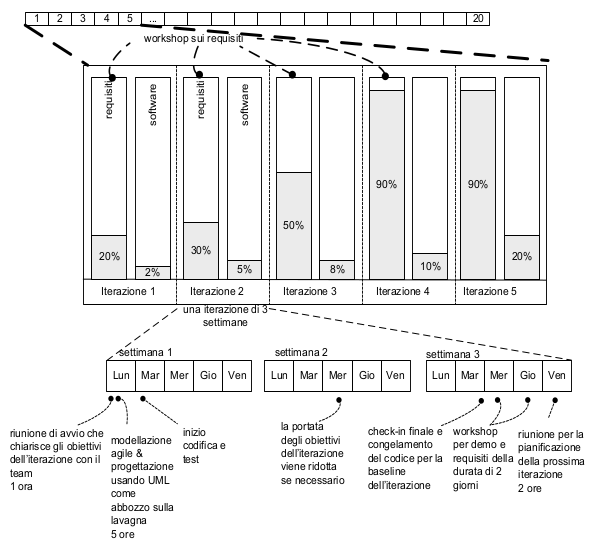
\includegraphics[scale=0.7]{img/ms7.png}
\end{center}
\newpage
vediamo un'altra rappresentazione del ciclo di sviluppo:
\begin{center}
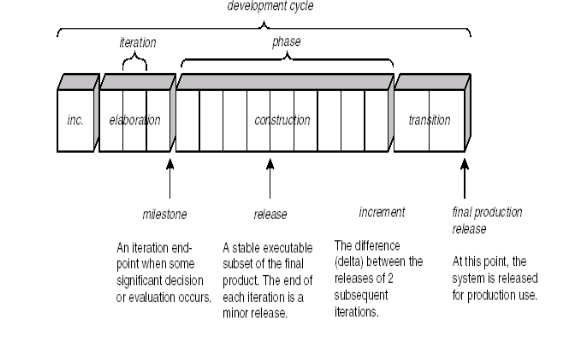
\includegraphics[scale=0.65]{img/ms8.png}
\end{center}
vediamo anche un'immagine per rappresentare l'organizzazione del processo, con fasi, iterazioni e "discipline":
\begin{center}
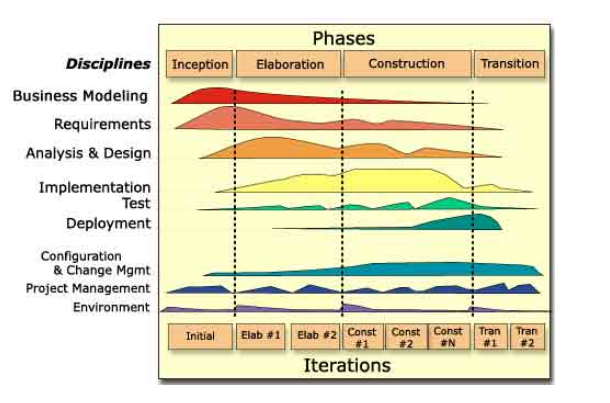
\includegraphics[scale=0.65]{img/ms9.png}
\end{center}
tra le discipline troviamo analisi e progettazione
%approfondire su libro
Si hanno le seguenti caratteristiche principali per l'UP:
\begin{itemize}
\item è iterativo e incrementale
\item si concentra sul modello invece che sul linguaggio naturale
\item è centrato sull'architettura
\end{itemize}
\subsection{Processo Scrum}
Iniziamo con un'immagine che rappresenta questo metodo agile:
\begin{center}
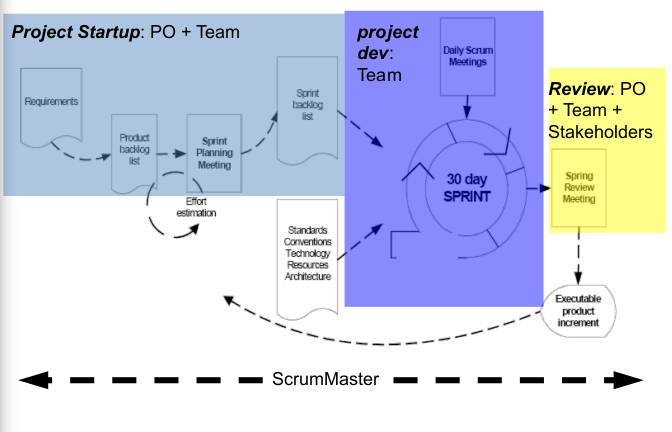
\includegraphics[scale=0.65]{img/ms10.png}
\end{center}
È un processo iterativo basato sull controllo dello stato di
avanzamento. Si hanno i seguenti principi fondamentali:
\begin{itemize}
\item \textbf{visibilità:} gli aspetti significativi del processo di sviluppo devono essere visibili a tutti e tutti gli aspetti devono essere chiari
\item \textbf{ispezione:} poter ispezionare frequentemente il lavoro fatto per verificare che si sta procedendo verso gli
obiettivi posti
\item \textbf{adattamento}, se si sta deviando dagli obiettivi, occorre un adattamento per minimizzare altre deviazioni. Deve essere svolto nel minor tempo possibile in caso di necessità
\end{itemize}
Si hanno i seguenti ruoli:
\begin{itemize}
\item \textbf{product owner} che si occupa della definizione delle
caratteristiche del progetto da sviluppare (1 sola
persona, e.g. committente, o altri...); gestisce il
Product Backlog. Lavora costantemente col team
\item \textbf{team:} dedicato allo sviluppo e rilascio del
prodotto attraverso incrementi successivi (da 3 a
7/8 membri)
\item \textbf{scrum master:} responsabile che lo SCRUM venga
applicato correttamente. Non è un project manager, fa da intermezzo tra team e product owner, collabora col team etc
\end{itemize}
Ecco un'immagine che rappresenta lo sviluppo con Scrum:
\begin{center}
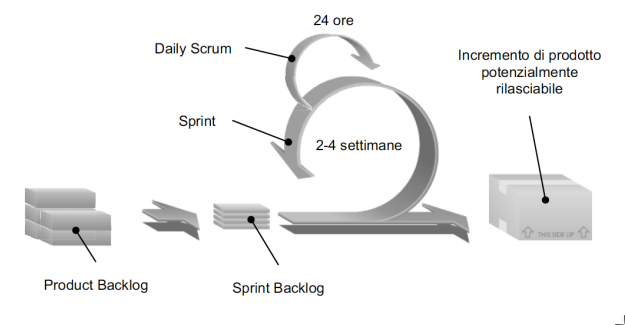
\includegraphics[scale=0.7]{img/ms11.png}
\end{center}
SI hanno quindi:
\begin{itemize}
\item releases brevi con sottoinsiemi consegnati velocemente
\item in ogni istante si hanno test eseguibili, non si ha logica duplicata e si ha un numero minimo di features
\item si ha \textit{refactoring }con miglioramento continuo
\item si un testo continuo e automatico, \textit{testing first}
\item si hanno due sviluppatori che lavorano insieme, \textit{pair programming}
\item il codice è proprietà del team e non del singolo dev, \textit{collective owbership}
\item si hanno check-in frequenti e integrazioni continue, \textit{continuous integration}
\item il cliente lavora col team
\end{itemize}
\end{document}